\section{CURSO DE INTRODUCCIÓN A LA ELECTROSTÁTICA}

Las actividades descriptas en esta sección, que se están desarrollando en un curso de Física 2 de la Universidad Tecnológica Nacional - Facultad Regional Avellaneda (UTN FRA), están fuertemente inspiradas en el curso de mecánica analítica \cite{bettachini_CLADI_2022} presentado en la sección anterior. La principal diferencia con dicho curso de mecánica, además de los temas estudiados, es el nivel de avance en sus carreras de las y los estudiantes en sendos cursos. En la materia Física 2 nos encontramos con estudiantes que poseen pocos o nulos conocimientos tanto de programación como de cálculo numérico. Entonces, en este caso, es importante sostener como premisa que el código sea sólo una herramienta que asiste a una mejor adquisición de los conceptos de la materia impartida, y que la comprensión del código no se transforme en una dificultad extra. Con este objetivo, las numerosas e intrincadas líneas de código para cálculos complejos y generación de figuras, están encapsuladas en funciones de bibliotecas del paquete {\tt frautnEM} (\url{https://github.com/frautn/frautnEM}), diseñado específicamente para asistir a este curso, de forma que las y los estudiantes solo trabajen con pocas líneas de código sencillo. A su vez, el material que utilizan docentes y estudiantes de este curso está disponible para ser utilizado, descargado y adaptado libremente en el repositorio \url{https://github.com/frautn/F2-electromagnetismo}.\par\medskip

El material se presenta a las y los estudiantes dividido en módulos, mediante cuadernos Jupyter que se cargan en la plataforma Google Colaboratory, y que contienen breves explicaciones, ejemplos resueltos con código, y actividades propuestas para ser realizadas reutilizando el código de los ejemplos. Estos módulos asisten a estudiantes de un primer curso de electromagnetismo en la adquisición de conceptos sobre campo y potencial electrostático, distribuciones contínuas de carga, campo y equipotenciales en presencia de conductores, enteramente utilizando código Python. En poco tiempo se encuentran trabajando en ejercicios cuya resolución en papel está descartada, no necesariamente por su dificultad, sino también por el volumen de cálculos repetitivos que deberían ser realizados.\par\medskip

A modo de ejemplo, la Figura \ref{fig:anillo} muestra como las y los estudiantes generan líneas de campo de un anillo cargado con una distribución de carga no uniforme. La Figura \ref{fig:anillo}(a) es el código provisto con el cuaderno Jupyter para generar una lista de cargas puntuales que simulen una distribución contínua con forma de anillo. Copiando este código, el o la estudiante solo debe modificar la función que calcula la carga en cada ángulo, escribiéndola en un formato familiar, en este caso como {\tt a*cos(2*t)}, siendo {\tt t} el ángulo, el radio del anillo y el número de cargas puntuales utilizadas para representar al anillo.  

\textcolor{red}{Se analizan las líneas de campo y las equipotenciales de distribuciones de cargas arbitrarias, como la mostrada en la figura 1, o incluso visualizaciones en 3 dimensiones, tareas imposibles de implementar si se trabajara en papel. En la misma figura se destaca la simplicidad con la que los estudiantes pueden generar dichos gráficos, mediante el llamado a una única función diseñada específicamente para este curso. A lo largo de toda la experiencia, los estudiantes solo necesitan modificar códigos sencillos.}\par\medskip

Figura: Código simple que genera líneas de campo.




Ver Figura \ref{fig:anillo}.

\begin{figure}[h]
	\centering
	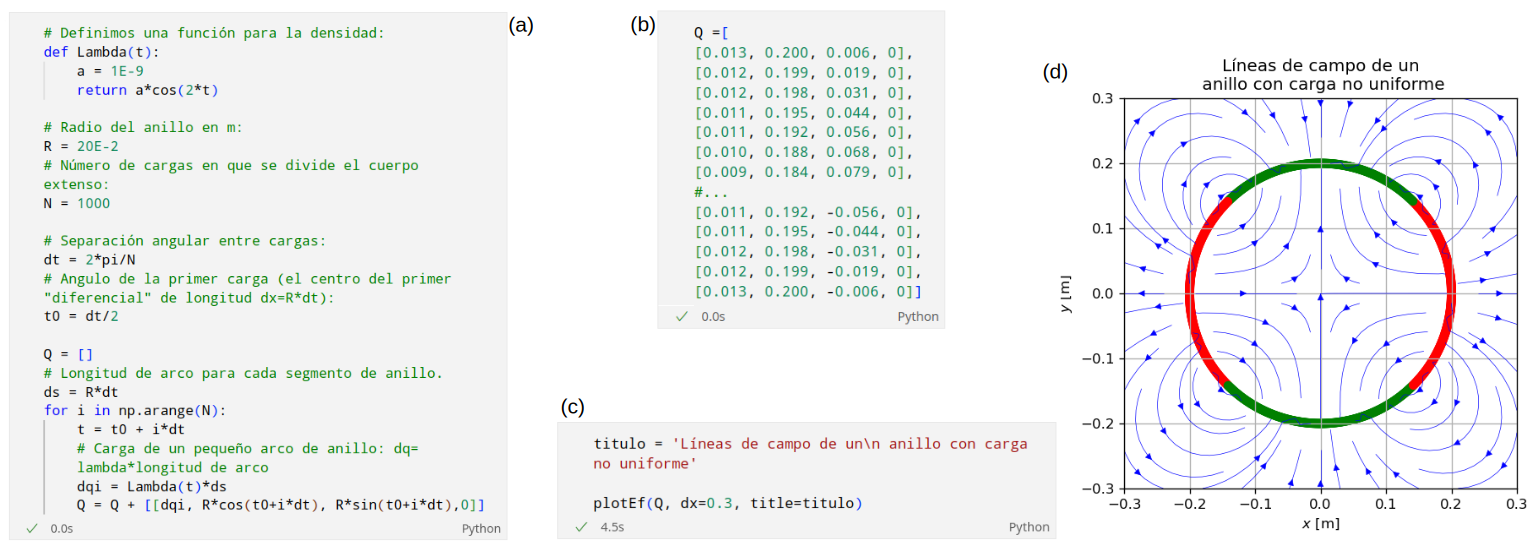
\includegraphics[width=160mm]{imagenes/anillo-variable.png}
	\caption{(a) Código para generar una lista de cargas puntuales que representen un anillo con carga variable. (b) La misma lista puede ser generada en una planilla de cálculo e ingresada manualmente. (c) Código muy breve y sencillo para generar las líneas de campo de esta distribución compleja. (d) La figura generada por la función {\tt plotEf()}.}
    \label{fig:anillo}
\end{figure}




Salir del plano. Ver Figura \ref{fig:superficies}.

\begin{figure}[h]
	\centering
	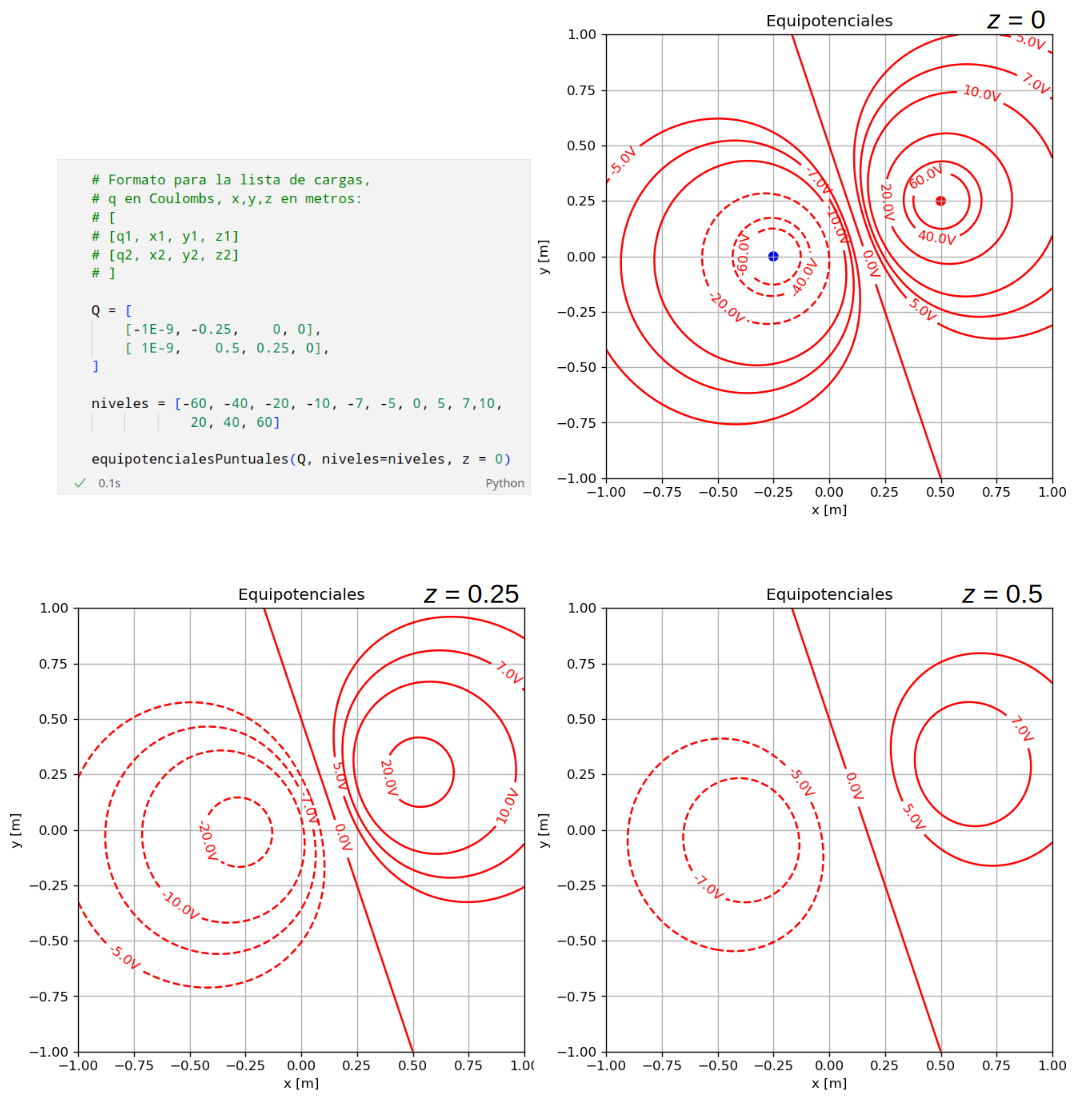
\includegraphics[width=160mm]{imagenes/equipotenciales_superficies.png}
	\caption{Con una simple línea de código se pueden estudiar las curvas equipotenciales resultantes de la intersección de las superficies equipotenciales con planos a diferentes alturas ($z = 0$ y $z = 0.5$) respecto de las cargas.}
    \label{fig:superficies}
\end{figure}

Con esta metodología, los estudiantes pueden:
\begin{itemize}
\item repasar lo trabajado en clases previas y adquirir nuevos conceptos sobre campo y potencial eléctrico;
\item acostumbrarse a que las distribuciones contínuas de carga eléctrica se pueden analizar como formadas por numerosas cargas puntuales, comprobando que se obtienen resultados muy aproximados a los resultados exactos que se obtienen usando fórmulas conocidas, como pueden ser la del campo eléctrico de esferas, líneas o planos cargados;
\item \textcolor{blue}{no trabarse con integrales que no dominan: más problemas en menos tiempo, más práctica para incorporación de conceptos, velocidad y facilidad para analizar variando parámetros;} 
\item reutilizar y adaptar código para experimentar con problemas cada vez más complejos, incluso no solo entre los propuestos en esta materia, sirviendo como una herramienta que se pueda aprovechar en otros contextos.
\end{itemize}
 
En el caso de los docentes, entre sus posibilidades se encuentran:
\begin{itemize}
    \item incluir en sus propuestas la resolución y el análisis de problemas que suelen estar descartados en una clase de pizarrón, debido a la dificultad de su abordaje (como es el caso del trabajo en 3 dimensiones) o a la longitud de los cálculos, aprovechando la reutilización de código;
	\item no destinar excesivo tiempo (de docentes y de estudiantes) repitiendo cálculos pesados, como por ejemplo las integrales múltiples relacionadas a distribuciones contínuas de cargas, y destinar ese tiempo al análisis de un mayor número de situaciones.
\end{itemize}


\textcolor{red}{Módulo 6 - Trabajo final: Se pide la resolución de un problema que involucre más de una de las herramientas usadas anteriormente, y se provee un cuaderno Jupyter en forma de plantilla para facilitar el inicio del trabajo.}

Extra: Aprovechar las posibilidades de cálculo simbólico que provee la biblioteca SymPy (Meurer et al., 2017) de Python para obtener soluciones exactas a problemas que involucran integrales múltiples complicadas y herramientas de análisis que aún no manejan.\par
\textcolor{red}{Módulo 4 - Distribuciones de carga contínuas (parte 2): Se obtienen soluciones exactas de configuraciones con distribuciones contínuas, utilizando la biblioteca Sympy para el cálculo de las integrales y los gradientes. En la figura 2 se muestra a modo de ejemplo el cálculo del campo generado por un segmento de carga. Notar que se obtiene el resultado del campo en cualquier posición, no solo en los ejes de simetría, que es una limitación usual al trabajar en papel.}\par
Conductores, simulación de la práctica de laboratorio.\par
\textcolor{red}{Módulo 5 - Campos y equipotenciales en presencia de conductores: La teoría involucrada para obtener equipotenciales cuando se tienen conductores con carga superficial no uniformes no forma parte de un curso de este nivel. Sin embargo, el análisis de los resultados sí puede incluirse como tarea. En particular, en este curso en el cual se está llevando a cabo la experiencia, los estudiantes realizan una práctica de laboratorio donde mapean el voltaje en una cuba que contiene electrodos extensos mantenidos a potencial constante, para luego estimar las curvas equipotenciales y las líneas de campo correspondientes. Por lo tanto, los análisis que los estudiantes realicen en este módulo son muy similares a dicha tarea de laboratorio. El código necesario para generar los gráficos está esencialmente provisto en bibiliotecas, por lo que los estudiantes sólo deben familiarizarse con la forma de presentar la geometría de los conductores.}\par\medskip  

Conclusiones:\par

“Since the notebooks are interactive, students can change the values of variables in an equation and immediately see what happens. That gives them a better sense of the physical reality underlying the equations,” 
